\section{Diagrama de flujo (firmware)}
\label{sec:diag_flujo}
A continuación se presenta el Diagrama de flujo correspondiente al Menú principal del proyecto. A través de este, que funciona como interfaz con el Usuario, se puede seleccionar los distintos modos de operación que puede ejecutar el microcontrolador.

\begin{itemize}
\item Seno: generación de una señal senoidal precargada en memoria del programa (ROM), con una Frecuencia y Amplitud prefijadas.
\item Dientes de Sierra: generación de una señal Dientes de Sierra, a partir de una función implementada en Assembly, con una Frecuencia y Valor Pico prefijados.
\item Matlab: el programa abre un canal de comunicación de transmisión Serie entre Matlab y el Microcontrolador, donde este último recibe datos, los almacena en RAM, procesa y genera la salida con los datos acondicionados entre 0 y 255 valores.
\item Intensidad: Este modo de operación permite al Microcontrolador medir la intensidad lumínica de las ramas del Interferómetro. Esto se hace mediante un fotodiodo en serie con una resistencia, la cual esta conectada al conversor Analogico-Digital interno del Microcontrolador. 
\end{itemize}

Las señales se generaran de forma continuada hasta que el usuario detiene el proceso mediante una Interrupción Externa activada al presionar un pulsador, la cual salta el programa al Inicio del Menú.
Dichas señales se generan en un Puerto establecido como salida, el cual tiene conectado un conversor Digital-Analógico (DAC).

\begin{figure}[H]
  \centering
  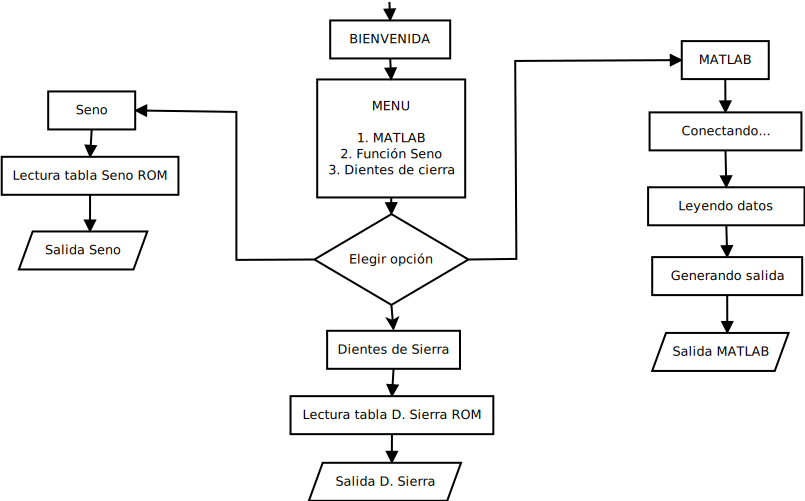
\includegraphics[width=1.0\textwidth]{images/flujo_menu_informe_v1.png}
  \caption{Diagrama de flujo del menú principal.}
  \label{fig:Diagrama de flujo}
\end{figure}